%  This is a LaTex file.

%  Homework for the course "AMath 585:  Applied Linear Algebra and Numerical Analysis", 
%  Autumn quarter, 2009, Anne Greenbaum.


%   A latex format for making homework assignments.


\documentclass[letterpaper,12pt]{article}

%          The page format, somewhat wider and taller page than in art12.sty.

\topmargin -0.1in \headsep 0in \textheight 8.9in \footskip 0.6in
\oddsidemargin 0in  \evensidemargin 0in  \textwidth 6.5in
\usepackage{graphicx}
\usepackage{listings}
\usepackage{caption}
\usepackage{subcaption}
\usepackage{color}
\usepackage{float}
\definecolor{keywords}{RGB}{255,0,90}
\definecolor{comments}{RGB}{0,0,113}
\definecolor{red}{RGB}{160,0,0}
\definecolor{green}{RGB}{0,150,0}
\definecolor{codegreen}{rgb}{0,0.6,0}
\definecolor{codegray}{rgb}{0.5,0.5,0.5}
\definecolor{codepurple}{rgb}{0.58,0,0.82}
\definecolor{backcolour}{rgb}{0.95,0.95,0.92}
\definecolor{brown}{rgb}{0.59, 0.29, 0.0}
\definecolor{beaublue}{rgb}{0.74, 0.83, 0.9}
\definecolor{orange}{rgb}{1.0, 0.5, 0.0}
\definecolor{darkslategray}{rgb}{0.18, 0.31, 0.31}
\definecolor{deepblue}{rgb}{0,0,0.5}
\definecolor{deepred}{rgb}{0.6,0,0}
\definecolor{deepgreen}{rgb}{0,0.5,0}
\lstdefinestyle{myMatlabstyle}{
	language=Matlab,
	backgroundcolor=\color{white},   
	commentstyle=\color{codegreen},
	keywordstyle=\color{blue},
	identifierstyle=\color{brown},
	numberstyle=\tiny\color{codegray},
	stringstyle=\color{orange},
	basicstyle=\footnotesize,
	breakatwhitespace=false,         
	breaklines=true,                 
	captionpos=b,                    
	keepspaces=true,                 
	numbers=left,                    
	numbersep=5pt,                  
	showspaces=false,                
	showstringspaces=false,
	showtabs=false,                  
	tabsize=2
}
\lstdefinestyle{myPythonstyle}{
	language=Python, 
	basicstyle=\ttfamily\small, 
	keywordstyle=\color{blue},
	backgroundcolor=\color{white}, 
	commentstyle=\color{green},
	stringstyle=\color{red},
	showstringspaces=false,
	%identifierstyle=\color{brown},
	breaklines=true, 
}
\lstset{language=Matlab,frame=single}
\lstset{language=Python,frame=single}
\usepackage{epsfig}         % to insert PostScript figures

\begin{document}


%          Definitions of commonly used symbols.



%          The title and header.


\begin{center}
\large
Assignment 3.
\normalsize

Jithin D. George, No. 1622555
\end{center}

\noindent
Due Monday, Jan. 29.

\vspace{.5cm}

\begin{enumerate}
\item (nonlinear pendulum)
\begin{enumerate}
\item Write a program to solve the boundary value problem for the nonlinear pendulum 
as discussed in the text.  See if you can find yet another solution for the boundary
conditions illustrated in Figures 2.4 and 2.5.  


{\bf Solution:}

\begin{figure}[H]

\centering
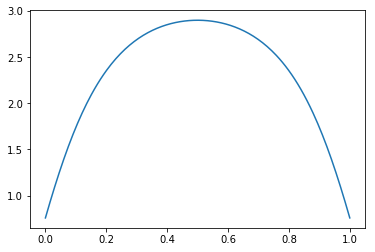
\includegraphics[width=0.5\textwidth]{311.png}


\caption{Initial condition of 0.7cos(t)+20sin(t)}
\label{fig:figure3}

\end{figure}

	\begin{lstlisting}[style=MyPythonstyle]
def tridiag(a, b, c, k1=-1, k2=0, k3=1):
    return np.diag(a, k1) + np.diag(b, k2) + np.diag(c, k3)
    
def mat(thetavec):
    N = len(thetavec)
    h =2*np.pi/N
    a1 = np.append([0.7],thetavec[:-1])
    a2 = np.append(thetavec[1:],[0.7])
    b = -2*thetavec+ a1+a2 + (h**2)* np.sin(thetavec)
    return b


def jacobian(thetavec):
    N = len(thetavec)
    h =2*np.pi/N
    a = np.ones(N-1)
    b = -2  + (h**2)* np.cos(thetavec)
    return tridiag(a,b,a)  


N=200
x = np.linspace(0,1,N)
thetavec = 0.7*np.cos(x)+2*np.sin(x)
for i in range(40):
    b = -mat(thetavec)
    A = jacobian(thetavec)
    delta = np.linalg.solve(A,b)
    thetavec += delta
    
plt.plot(x,thetavec)
\end{lstlisting}


\item Find a numerical solution to this BVP with the same general behavior as seen
in Figure 2.5 for the case of a longer time interval, say, $T = 20$, again with $\alpha =
\beta = 0.7$.  Try larger values of $T$.  What does $\max_i \theta_i$ approach as $T$ is
increased?  Note that for large $T$ this solution exhibits ``boundary layers''.

{\bf Solution:}

\begin{figure}[H]

\centering
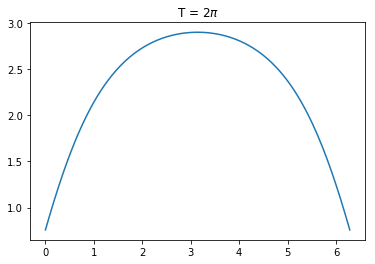
\includegraphics[width=.3\textwidth]{312a.png}\hfill
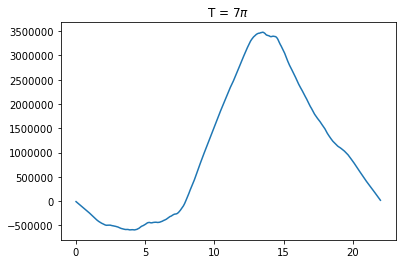
\includegraphics[width=.3\textwidth]{312b.png}\hfill
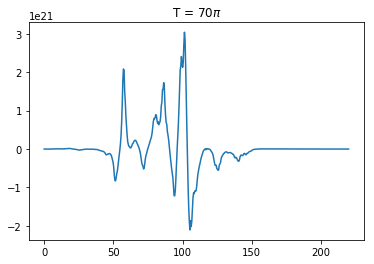
\includegraphics[width=.3\textwidth]{312c.png}

\caption{Solutions at t = 2$\pi$,7$\pi$ and 70$\pi$}
\label{fig:figure3}
\end{figure}

\end{enumerate}

As T increases, maximum value of theta goes to infinity.

\item (Gerschgorin's theorem and stability)
Consider the boundary value problem
\[
- u_{xx} + ( 1 + x^2 ) u = f ,~~0 \leq x \leq 1 ,
\]
\[
u(0) = 0 ,~~u(1) = 0.
\]
On a uniform grid with spacing $h = 1/(m+1)$, the following set of difference equations
has local truncation error $O( h^2 )$:
\[
\frac{2 u_i - u_{i+1} - u_{i-1}}{h^2} + (1 + x_i^2 ) u_i = f( x_i ) ,~~i=1, \ldots , m .
\]
\begin{enumerate}
\item
Use Gerschgorin's theorem to determine upper and lower bounds on the
eigenvalues of the coefficient matrix for this set of difference equations.

{\bf Solution:}

The global error is related to the local error by 
\[A e = \tau\]
Where A is 
\[ \frac{1}{h^2} \left( \begin{array}{cccccc}
2 + (1 + x_0^2 )h^2 & -1 &        &        &    &  \\
-1  & 2 + (1 + x_i^2 )h^2 & -1      &        &    &  \\
   & -1  & \ddots & \ddots &     & \\
   &    & \ddots & \ddots & \ddots   & \\
   &    &        & -1      & 2 + (1 + x_i^2 )h^2 & -1 \\
      &    &        &       & -1 & 2 + (1 + x_n^2 )h^2 \\
   \end{array} \right)
\]
By Gerschgorin's theorem,
\[|\lambda -(2 + (1 + x_i^2 )h^2)| \leq 2\]
\[- 2\leq \lambda -(2 + (1 + x_i^2 )h^2) \leq 2\]
\[ (1 + x_i^2 )h^2\leq \lambda  \leq 4 + (1 + x_i^2 )h^2\]
\[ h^2\leq \lambda  \leq 4 + 2h^2\]
\[ 1\leq \frac{\lambda}{h^2}  \leq \frac{4}{h^2} + 2\]

Thus, the eigenvalues of the coefficient matrix lie in 1 and $\frac{4}{h^2} + 2$
\item
Show that the $L_2$-norm of the {\em global error} is of the same order as the local
truncation error.

{\bf Solution:}


\[e = A^{-1}\tau\]
\[||e||_2 = ||A^{-1}\tau||_2 \leq ||A^{-1}||_2||\tau||_2 \leq \lambda(A^{-1})_{max}||\tau||_2 \]
Since
\[ 1\leq \lambda(A)  \leq \frac{4}{h^2} + 2\]
\[ \frac{h^2}{4 + 2h^2} \leq \lambda(A^{-1}) \leq 1 \]
Thus,
\[||e||_2 \leq ||\tau||_2\]

\end{enumerate}

\newpage
\item (Richardson extrapolation)
\begin{enumerate}
 \item 

Use your code from problem 6 in assignment 1, or download the code from the
course web page to do the following exercise.  Run the code with $h = .1$
($10$ subintervals) and with $h=.05$ ($20$ subintervals) and apply
Richardson extrapolation to obtain more accurate solution values on the
coarser grid.  Record the $L_2$-norm or the $\infty$-norm of the error
in the approximation obtained with each $h$ value and in that obtained
with extrapolation.

{\bf Solution:}

Using the infinity norm.

\begin{tabular}{rr}
\hline
    h &      Error \\
\hline
 0.1  & 0.00222556 \\
 0.05 & 0.0005504  \\
\hline
\end{tabular}

Using Richardson's extrapolation, we get the error = 7.9865541829916443e-06 which is less than our previous errors.

\item
Suppose you assume that the coarse grid approximation is piecewise
linear, so that the approximation at the midpoint of each subinterval
is the average of the values at the two endpoints.  Can one use Richardson
extrapolation with the fine grid approximation and these interpolated
values on the coarse grid to obtain a more accurate approximation at
these points?  Explain why or why not?

{\bf Solution:}

	\begin{lstlisting}[style=MyPythonstyle]
Y1 = prob_6([rho,f,u],x,1/10)
Y2 = prob_6([rho,f,u],x,1/20)

def interplot(Y):
    j=[Y[0]]
    for i in range(1,len(Y)):
        j.append(0.5*(Y[i]+Y[i-1]))
        j.append(Y[i])
    return j
Ynew = interplot(Y1)
rich2 =( 4*Y2-Ynew)/3
eee=U-rich2
error+=[np.linalg.norm(eee,np.inf)]
\end{lstlisting}

The error obtained using Richardson's extrapolation in this way is 0.00083991977137813927.
This is worse than the error when we used h = 0.05. The reason is that the solution is $(1-x)^2$ which is quadratic. So, using a piecewise linear interpolation would create errors.


\end{enumerate}

\item
Write down the Jacobian matrix associated with Example 2.2 and the 
nonlinear difference equations (2.106) on p.~49.  Write a code to solve these
difference equations when $a=0$, $b=1$, $\alpha = -1$, $\beta = 1.5$, and $\epsilon = 0.01$.
Use an initial guess of the sort suggested in the text.
Try, say, $h=1/20$, $h=1/40$, $h=1/80$, and $h=1/160$, and turn in a plot of your results.


{\bf Solution:}
\begin{figure}[H]

\centering
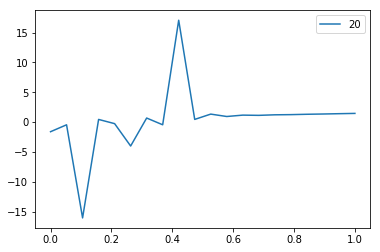
\includegraphics[width=.45\textwidth]{341.png}\hfill
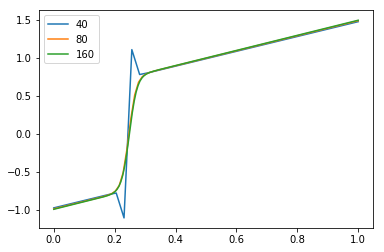
\includegraphics[width=.45\textwidth]{342.png}\hfill


\caption{Boundary layers at N = 20 and N= 40, 80 and 160}
\label{fig:figure3}

\end{figure}

	\begin{lstlisting}[style=MyPythonstyle]
def tridiag(a, b, c, k1=-1, k2=0, k3=1):
    return np.diag(a, k1) + np.diag(b, k2) + np.diag(c, k3)
    
def mat2(thetavec,h,e=0.01):
    a1 = np.append([-1],thetavec[:-1])
    a2 = np.append(thetavec[1:],[1.5])
    b = e*(-2*thetavec+ a1+a2) + thetavec*(0.5*h*(a2-a1)-h**2)
    return b

def jacobian2(thetavec,h,e=0.01):
    a1 = np.append([-1],thetavec[:-1])
    a2 = np.append(thetavec[1:],[1.5])
    b = -2*e  + (0.5*h*(a2-a1)-h**2)
    return tridiag(e-0.5*h*thetavec[1:],b,e+0.5*h*thetavec[:-1])   
N=60
h =1/N
e=0.01
w_0 =1.5
x_0 = 0.25
x= np.linspace(0,1,N)

thetavec = x - x_0 +w_0*np.tanh(w_0*(x-x_0)/(2*e))
for i in range(100):
    b = -mat2(thetavec,h,e)
    A = jacobian2(thetavec, h,e)
    delta = np.linalg.solve(A,b)
    thetavec += delta
plt.plot(x,thetavec)
\end{lstlisting}


\end{enumerate}

\end{document}

